\documentclass{article}
\usepackage{graphicx}
\usepackage[fleqn]{amsmath}
\usepackage[a4paper, margin=2cm]{geometry}
\usepackage{pdfpages}

\newcommand{\comment}[1]{}
\begin{document}
\title{Practical 3}
\author{Janco Spies, u21434159}
\maketitle
\section*{Task 2}
\begin{itemize}
    \item[2.1] A way to handle this situation using procedural programming is to 
                have the function return null and then make the client check if
                the returned pointer is null before proceeding.
    \item[2.2] A way to handle this situation using an object-oriented approach 
                is to add a new class that represents a blank object similar to
                the constant "NaN" for number variables. This class will then be 
                created and returned to the client.
    \item[2.4] 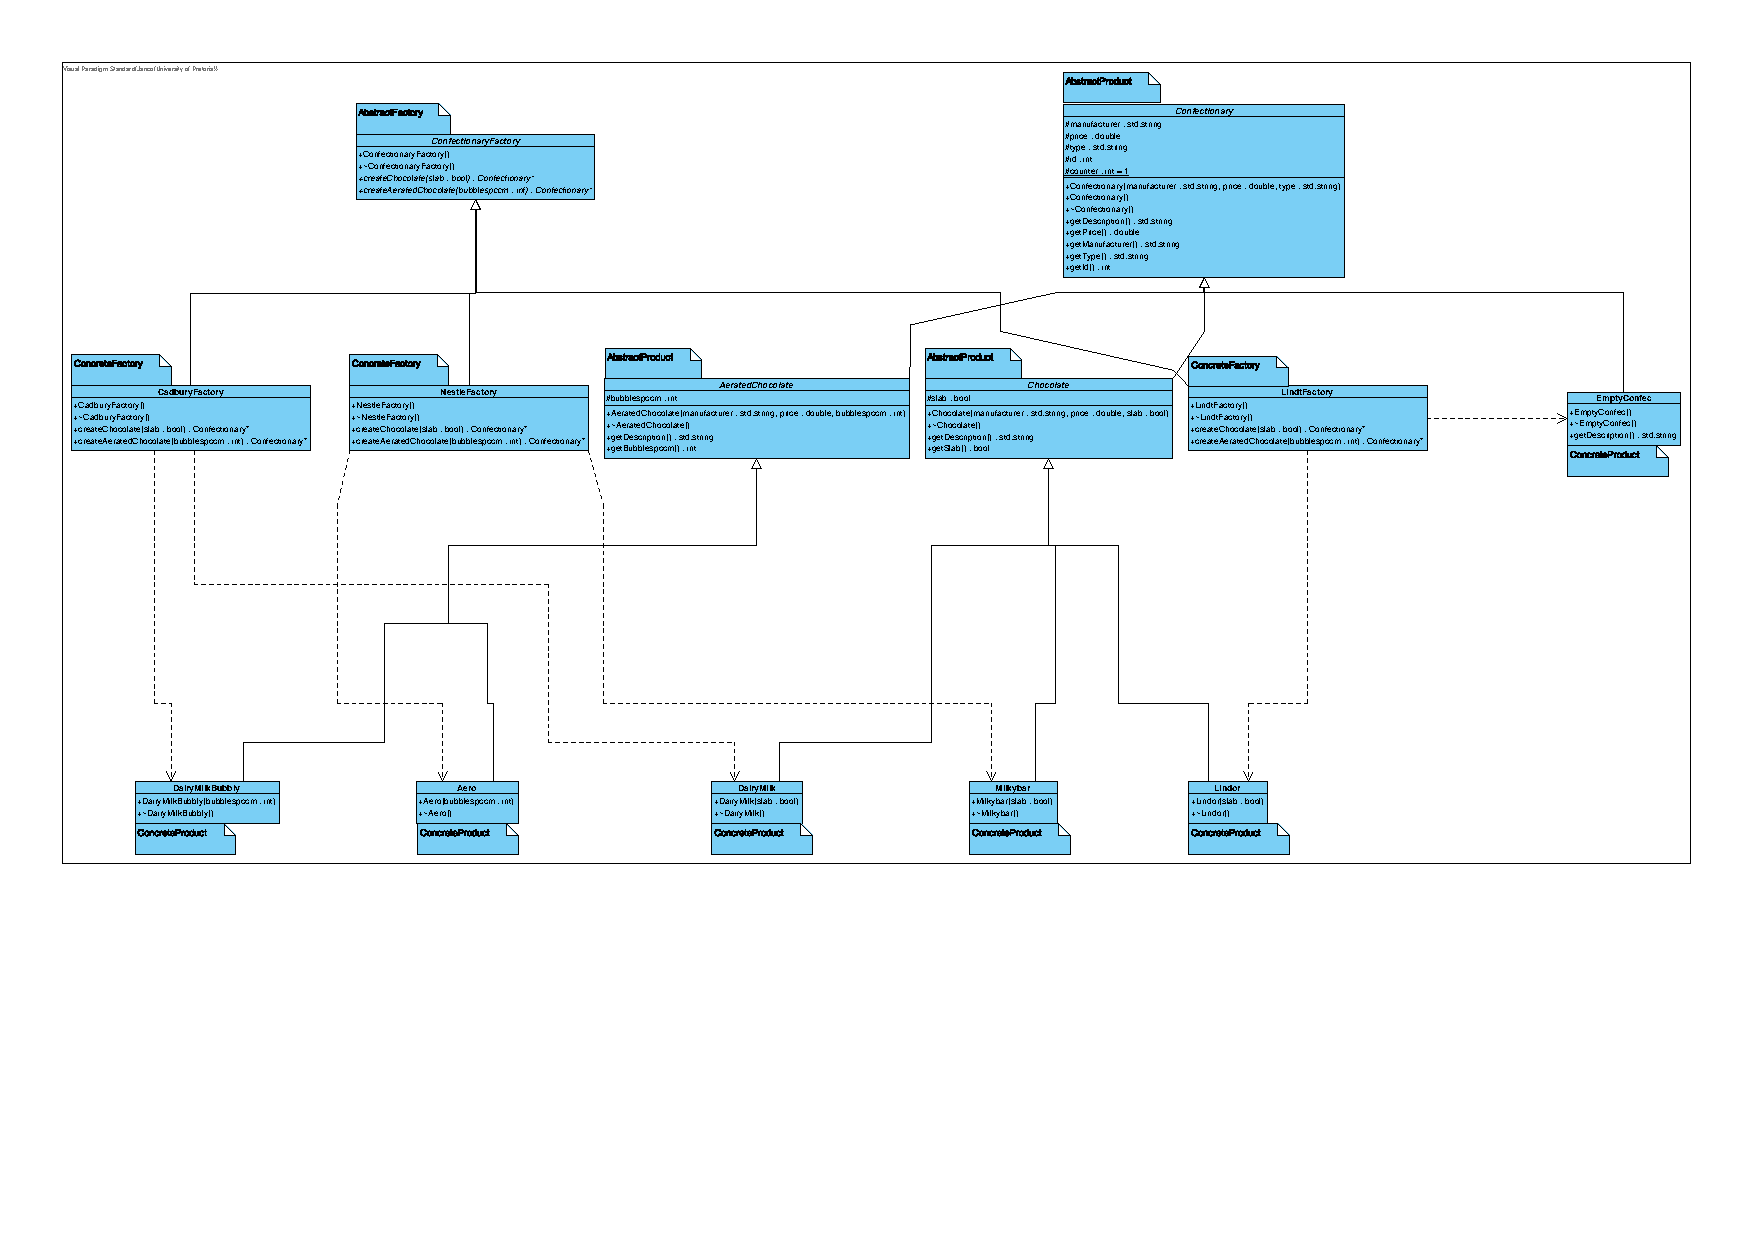
\includepdf[pages=-]{Task2.pdf}
\end{itemize}
\end{document}